\documentclass[]{article}
\usepackage{caption,subcaption,graphicx,float,url,amsmath,amssymb,amsthm,tocloft,cancel,thmtools,gensymb,braket}
\usepackage[toc,nonumberlist]{glossaries}
\usepackage{glossaries-extra}
\newcommand\numberthis{\addtocounter{equation}{1}\tag{\theequation}}

\newtheorem{thm}{Theorem}
\newtheorem{defn}[thm]{Definition}
\newtheorem{cor}[thm]{Corollary}
\newtheorem{lemma}[thm]{Lemma}
\graphicspath{{figs/}}
\widowpenalty10000
\clubpenalty10000
\setcounter{tocdepth}{2}

%opening
\title{Theoretical Minimum\\Particle Physics 2\\Standard Model}
\author{}

\begin{document}

\maketitle
\tableofcontents
\listoffigures
\begin{abstract}

\end{abstract}

\section{Particles fields and forces}

There is a triangle of concepts:
\begin{itemize}
	\item particles (quanta of fundamental fields)\footnote{We are going to have to think very hard about what is an elementary particles and what is composite always be frustrated, always find some slipper region why your definition did not work.}
	\item Fields
	\item Forces
\end{itemize}

\begin{figure}[H]
	\begin{center}
		\caption{Triangle}
		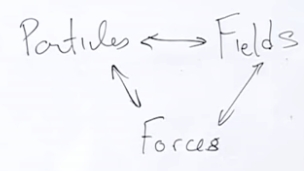
\includegraphics[width=0.5\textwidth]{ParticlesFieldsForces}
	\end{center}
\end{figure}

Consider two electric charges

\begin{align*}
E=&\int (e_1 \vec{E_1})^2 dV\\
E=&\int (e_2 \vec{E_2})^2 dV\\
E=&\int (e_1\vec{E_1}+e_2 \vec{E_2})^2 dV\\
=&\int \underbrace{(e_1E_1)^2}_\text{self energy}+ \underbrace{(e_2\vec{E_2})^2}_\text{self energy} + \underbrace{2e_1e_2\vec{E_1}.\vec{E_2}}_\text{interesting term}
\end{align*}

The last term is proportional to the charges.
\begin{itemize}
	\item  If they are so far away that $\vec{E_1}$ is negligible near second charge there will be no perceptible effect.
	\item If the particles are close we will get a contribution from $\vec{E_1}.\vec{E_2}$. This turns out to be the Coulumb force. 
\end{itemize}

The force comes from the distortion of the field: this is a \emph{purely field view of forces}. If fields give rise to forces, and particles are quanta of fields, there must be a way to think of forces coming from particles.

\url{https://youtu.be/Igl8hE3Eac0?t=821}

\subsection{Renormalization}

\subsection{The equivalence of particles, fields, and forces}

\subsection{The particle zoo}

\section{Quantum chromodynamics}



\section{Group theory – part 1}



\section{Group theory – part 2}



\section{Gauge fields and symmetry}



\section{The weak interaction}



\section{Spontaneous symmetry breaking and Goldstone bosons}



\section{The Higgs field}






\section{The Higgs field and fermions}



\section{Renormalization and the running of coupling constants}







\end{document}
